
\chapter{Planar graphs}
		A \textit{plane graph} is a pair $G = (V,E)$ where $V \subseteq \mathbb{R}^2$ such that:
		\begin{enumerate}
			\item Every edge is an arc linking two distinct vertices
			\item $\forall e \in E$, the interior $\text{int}(e)$ (the arc, minus the two vertices) contains no vertex of $G$ nor any point from edges $f \in E - \{ e \}$.
			\item Every pair of vertices is linked by at most one edge.
		\end{enumerate}
		Without the third condition, this could be a plane multi-graph (possibly involving "parallel" edges).\\
		
		A plane graph defines a corresponding abstract graph $G$. With a slight abuse of notation, we will write $G$ both for the abstract graph and for the corresponding subset of the plane: $V \cup \Large{\cup_{e \in E}} e \subseteq \mathbb{R}^2$.\\
		
		The \textit{faces} of $G$ are the regions of $\mathbb{R}^2 \setminus G$. Exactly one of these faces is unbounded and is called the \textit{outer face}. The other faces are called \textit{inner faces}. \\
		
		All acyclic plane graphs will have only an outer face. As soon as there is a cycle, there will be at least one inner face. In other words: a plane graph has only one face (the outer face) $\iff$ it is a forest.

\bigskip
$F(G) := |\text{face of }G|$\\
$\forall F \in F(G), \partial F$ is the boundary of $F$

		\subsection{Lemma 1}
		\textit{Let $F \in F(G)$. Then:}
		\begin{enumerate}
			\item $\partial F \subseteq G$
			\item \textit{$\forall e \in E(G)$, either $e \in \partial F$, or $\partial F \cap \text{int}(e) = \emptyset$}
			\item \textit{If $e \in E(G)$ is on a cycle $C \in G$, then $e$ is contained in the boundary of exactly two faces of $G$, one inside $C$ and the other outside $C$.}
			\item \textit{If $e \in E(G)$ is not included in any cycle, then $e$ appears in the boundary of exactly one face.}
		\end{enumerate}
		
		
		\subsection{Lemma 2}
		\textit{If $G$ is a 2-connected plane graph, then the boundary of every face is a cycle of $G$.\\}
		
		Some other properties:
		\begin{itemize}
			\item A graph is planar if it can be realised as a plane graph.
			\item A plane graph is \textit{maximally plane} if one cannot add any edge to it (while staying a plane graph).
			\item A plane graph is a \textit{plane triangulation} if every face is bounded by a triangle of the graph.
		\end{itemize}
		
		
		\subsection{Lemma 3}
		\textit{A plane graph on at least 3 vertices is maximally plane $\iff$ it is a plane triangulation}
		
		
		\subsection{Theorem 1: Euler's formula}
		\textit{Let $G$ be a connected plane graph with $n$ vertices, $m$ edges and $f$ faces. Then:}
		\begin{eqnarray}
			n - m + f = 2
		\end{eqnarray}
		\textit{Note that this formula works only for connected graphs.\\}
		
		Let's prove it with induction on $m$.
		\begin{enumerate}
			\item Base case: $m = n -1$ (as it's connected, it contains a spanning tree, it has $n - 1$ edges). In this case $G$ is a tree and $f = 1$. So $n - m + f = 2$.
			\item Inductive step: $m \geq n$. The connected graph is not a tree, then it has a cycle. Consider a cycle of $G$ and let $e \in E(C)$. The edge is on the cycle, so it's on the boundary of exactly two distinct faces of the graph $F_1, F_2 \in F(G)$. If we remove this edge from the graph, the graph stays connected but two faces merge so $f$ decreases by 1. So $f \rightarrow f -1$, $m \rightarrow m - 1$ and $n$ remains the same. Then $-m + f$ is constant and $n -m + f = 2$.
		\end{enumerate}
		
		\subsection{Corollary 1} 
		\textit{If $G$ is an $n$-vertex plane graph with $n$ being at least $3$, then $G$ has at most $3n - 6$ edges.\\}
		
		With my assumption WLOG that $G$ is maximally plane, i.e. $G$ is a plane triangulation. Let $m := |E(G)|$ and $f := |F(G)|$.
		\begin{eqnarray}
			3f = \sum_{F \in F(G)} 3 = 2m
		\end{eqnarray}
		If we look at every face in the triangulation, each edge will be counted two times as it is boundary to two faces. Hence:
		\begin{eqnarray}
			m = \frac{3}{2} f
		\end{eqnarray}
		And by Euler's formula (which we will use as we're considering a plane triangulation):
		\begin{eqnarray}
			n - m + f = 2
		\end{eqnarray}
		Thus 
		\begin{eqnarray}
			n - m + \frac{2}{3}m &=& 2 \\
			\implies n - \frac{1}{3} m &=& 2 \\
			\implies m &=& 3n - 6
		\end{eqnarray}
		
		\subsection{Corollary 2}
		\textit{$K_5$ is not planar.\\}
		
		$K_5$ has $n = 5$ vertices and $m = 10$ edges but $3n - 6 = 9 < 10$.
		
		
		\subsection{Lemma 3}
		\textit{If $G$ is an $n$-vertex plane graph ($n \geq 3)$ and has no triangle (i.e cycle of length 3 or 3 vertices that are pairwise adjacent), then $G$ has at most $2n - 4$ edges.\\}
		
		\subsection{Corollary 3}
		\textit{$K_{3,3}$ is not planar.\\}
		
		$K_{3,3}$ has $n = 6$ vertices and $m = 9$ edges: $2n - 4 = 8 < 9$.
		
		\subsection{Corollary 4}
		\textit{No planar graph contains $K_5$ or $K_{3,3}$ as a minor.}
		
		\subsection{Theorem 2: Kuratowski (1930)}
		\textit{A graph $G$ is planar $\iff$ $G$ it has neither $K_5$ nor $K_{3,3}$ as minor.\\}
		
		\begin{enumerate}
			\item $\implies$: already done.
			\item $\impliedby$: We first prove the statement in the case that $G$ is 3-connected. That is, we will show: "$G$ 3-connected and has neither $K_5$ or $K_{3,3}$ as minor $\implies$ $G$ is planar", by reduction on $|V(G)|$.
				\begin{enumerate}
					\item Base case: $|V(G)| = 4$. Then $G = K_4$ and is planar.
					\item Inductive step: $|V(G)| \geq 5$. By Tutte's theorem, there is an edge $xy \in E(G)$ such that when we contract (we get $G \setminus xy$), the graph is 3-connected. Note that $G \setminus xy$ has no $K_5$ nor $K_{3,3}$ minor (by transitivity of the minor relation), thus $G \setminus xy$ is planar by induction. Let $v_{xy}$ be the vertex resulting from the edge contraction. Consider a drawing of $G \setminus xy$ in the plane. The plane graph $(G \setminus xy) - v_{xy}$ is 2-connected. In particular, each face is bounded by a cycle of that graph. Let $C$ denote the cycle bounding the face where $v_{xy}$ was drawn.
\begin{figure}[H]
	\center
	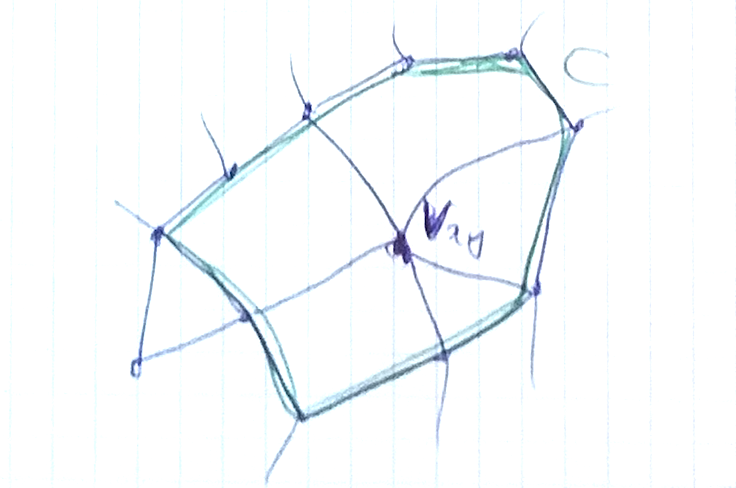
\includegraphics[height=5cm]{img/4-1.png}
\end{figure}

Then all neighbours of $v_{xy}$ in $G \setminus xy$ are on $C$. Let:
						\begin{eqnarray}
							X &:=& \{ v \in V(C) : vx \in E(G)\}\\
							Y &:=& \{ v \in V(C) : vy \in E(G) \}
						\end{eqnarray}
						Note that $|X| \geq 2$ and $|Y| \geq 2$, since $G$ is 3-connected.\\
						\begin{figure}[h]
	\center
	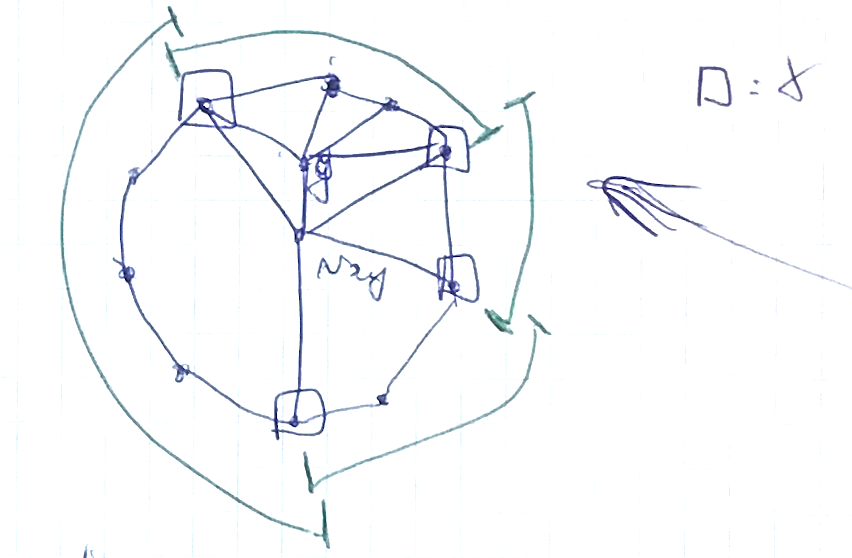
\includegraphics[height=5cm]{img/4-2.png}
\end{figure}

Consider the plane graph $H := (G \setminus xy) - \{ vy : v \in Y -X \}$. Note that all the remaining edges are at least adjacent to $X$.
						\begin{enumerate}
							\item Vertices of $X$ define intervals of $C$. One can see $H$ as a plane drawing of $G - y$ (where $v_{xy}$ plays the role of $x$). Our aim is to add $y$ to obtain a drawing of $G$.
							\item If there exists a single interval containing all of $Y$ then we can extend this drawing to a drawing  of $G$ by adding $y$ in the face made by the vertices of $Y$.
							\item Now let's assume this is not the case. We will show that this leads to a contradiction (and this $Y$ must be contained in a single interval).
								\begin{enumerate}
									\item $|X \cap Y| \geq 3$, then there is a $K_5$ minor in $G$.
									\begin{figure}[h]
	\center
	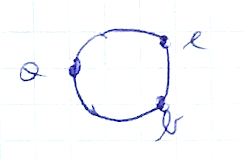
\includegraphics[width=0.3\linewidth]{img/4-3.png}
\end{figure}

Let $a,b,c \in X \cap Y$ be distinct. Consider the minor of $G$ obtained by contracting each of these three paths into edges.
			
			Then in that minor $\{ a,b,c,x,y \}$ are pairwise linked ($a,b,c$ are a triangle, $x$ and $y$ are both connected to all $a,b,c$). Hence $K_5$ is a minor of $G$. Contradiction.
									


									\item $|X \cap Y| \leq 2$, then there is a $K_{3,3}$ minor in $G$: 
									\begin{figure}[h]
	\center
	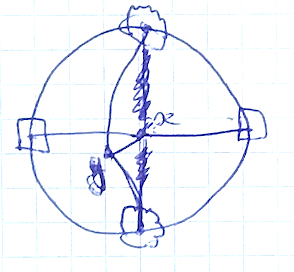
\includegraphics[width=0.3\linewidth]{img/4-4.png}
\end{figure}
								\end{enumerate}
						\end{enumerate} 
				\end{enumerate}
		\end{enumerate}
		
		\textit{Note this usual approach in graph theory: assume the graph has some connectivity, prove the theorem, then extend}
		
